\documentclass[a4paper]{article}

\usepackage{fullpage} % Package to use full page
\usepackage{parskip} % Package to tweak paragraph skipping
\usepackage{amsmath}
\usepackage{hyperref}
\usepackage{amsmath,amsfonts,amsthm} % Math packages
\usepackage{graphicx}
\usepackage{listings}
\usepackage{color}
\usepackage{float}
\definecolor{codegreen}{rgb}{0,0.6,0}
\definecolor{codegray}{rgb}{0.5,0.5,0.5}
\definecolor{codepurple}{rgb}{0.58,0,0.82}
\definecolor{backcolour}{rgb}{0.95,0.95,0.92}
\definecolor{brown}{rgb}{0.59, 0.29, 0.0}
\definecolor{beaublue}{rgb}{0.74, 0.83, 0.9}
\definecolor{orange}{rgb}{1.0, 0.5, 0.0}
\definecolor{darkslategray}{rgb}{0.18, 0.31, 0.31}
\def\Xint#1{\mathchoice
	{\XXint\displaystyle\textstyle{#1}}%
	{\XXint\textstyle\scriptstyle{#1}}%
	{\XXint\scriptstyle\scriptscriptstyle{#1}}%
	{\XXint\scriptscriptstyle\scriptscriptstyle{#1}}%
	\!\int}
\def\XXint#1#2#3{{\setbox0=\hbox{$#1{#2#3}{\int}$}
		\vcenter{\hbox{$#2#3$}}\kern-.5\wd0}}
\def\dashint{\Xint-}

% Swap the definition of \abs* and \norm*, so that \abs
% and \norm resizes the size of the brackets, and the 
% starred version does not.
\makeatletter
\let\oldabs\abs
\def\abs{\@ifstar{\oldabs}{\oldabs*}}
%
\let\oldnorm\norm
\def\norm{\@ifstar{\oldnorm}{\oldnorm*}}
\makeatother
\lstdefinestyle{mystyle}{
	backgroundcolor=\color{white},   
	commentstyle=\color{codegreen},
	keywordstyle=\color{blue},
	identifierstyle=\color{brown},
	numberstyle=\tiny\color{codegray},
	stringstyle=\color{orange},
	basicstyle=\footnotesize,
	breakatwhitespace=false,         
	breaklines=true,                 
	captionpos=b,                    
	keepspaces=true,                 
	numbers=left,                    
	numbersep=5pt,                  
	showspaces=false,                
	showstringspaces=false,
	showtabs=false,                  
	tabsize=2
}
\lstset{style=mystyle}
\newenvironment{mat}{\left[ \begin{array}{ccccccccccccc}}{\end{array}\right]}

\newcommand\bcm{\begin{mat}}
\newcommand\ecm{\end{mat}}

\title{AMATH 568: Problem Set 3}
\author{Jithin D. George, No. 1622555}
%\date{23/11/16}

\begin{document}

\maketitle
\begin{enumerate}

	
\item 
\[   r^3-r +\epsilon=0\]

\[r= r_0+ r_1 \epsilon + r_2 \epsilon ^2 +O(\epsilon^3)\]
\[r^3= r_0^3 + 3r_0^2r_1 \epsilon + (3r_0^2r_2+3r_0r_1^2)\epsilon^2 \]
\[   r^3-r +\epsilon=r_0^3-r_0 + (3r_0^2r_1-r_1+1) \epsilon + (3r_0^2r_2+3r_0r_1^2-r_2)\epsilon^2 \]


The exact solutions are 
\[r=0, 1,-1\]

For $r_0$=0,
\[ r_1 =1\]
\[ r_2 =0\]
\[r=  \epsilon  +O(\epsilon^3)\]
For $r_0$=1,
\[ r_1 =-\frac{1}{2}\]
\[ r_2 =-\frac{3}{8}\]
\[r= 1- \frac{1}{2} \epsilon + \frac{3}{8} \epsilon ^2 +O(\epsilon^3)\]

For $r_0$=-1,
\[ r_1 =-\frac{1}{2}\]
\[ r_2 =\frac{3}{8}\]
\[r= -1- \frac{1}{2} \epsilon -\frac{3}{8} \epsilon ^2 +O(\epsilon^3)\]

The first figure is for $\epsilon$ between -1 and 1. The second is between -2 and 2. The red circles represent the exact root. The first series around 0 is the starred line. The second series around 1 is the regular line and the third one around -1 is dashed line. 
	    \begin{figure}[H]
	    	\centering
	    	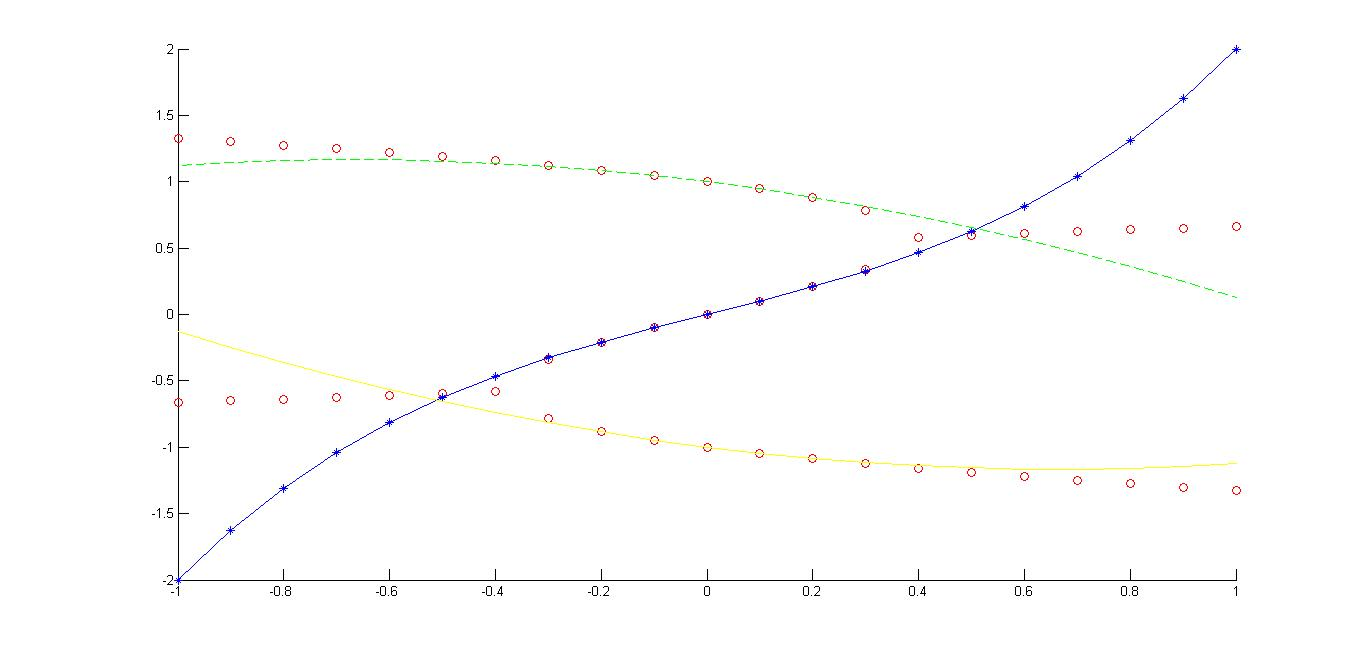
\includegraphics[width=12cm]{1to1}
	    	\caption{From -1 to 1 }
	    	
	    \end{figure}

	    \begin{figure}[H]
	    	\centering
	    	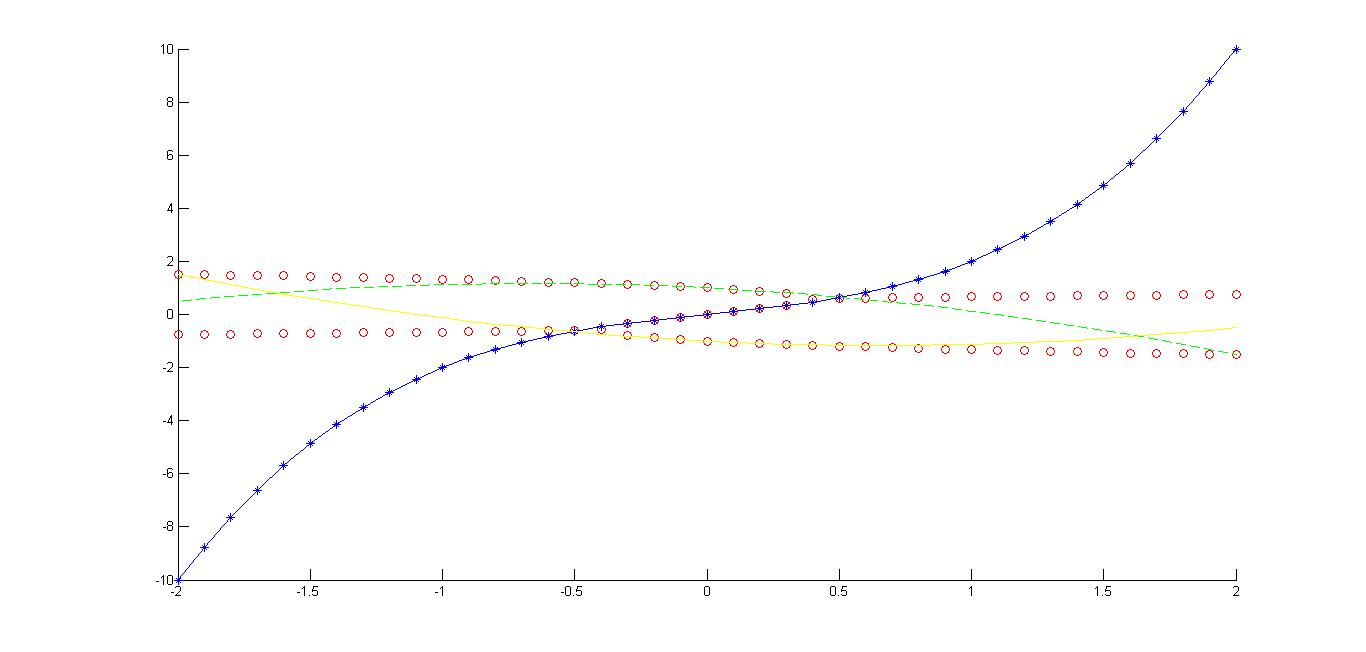
\includegraphics[width=12cm]{2to2}
	    	\caption{From -2 to 2 }
	    	
	    	\end{figure}

Thus we see that the series around the root 0 works well between -0.5 and 0.5. The series around the root 1 works well between -1 and 0.5. The series around the root -1 works well between -0.5 and 1.  	
	    	
\item
The main equation is 
\[(1+\epsilon)r^2-(4+\epsilon)r+4=0\]

\[r= r_0 +r_1 \epsilon +O(\epsilon^2)  \]
\[(1+\epsilon)r^2=(1+\epsilon)(r_0 +r_1 \epsilon)^2= (1+\epsilon)(r_0^2 +r_1^2\epsilon^2 +2r_0r_1\epsilon)= r_0^2 +r_1^2\epsilon^2 +2r_0r_1\epsilon + r_0^2\epsilon +r_1^2\epsilon^3 +2r_0r_1\epsilon^2 
\] \[ = r_0^2 +\epsilon(2r_0r_1+r_0^2)+\epsilon^2(r_1^2+2r_0r_1) +r_1^2\epsilon^3\]

\[(4+\epsilon)r =(4+\epsilon)(r_0 +r_1 \epsilon)= 4 r_0+ (4 r_1 +r_0)\epsilon +r_1 \epsilon^2 \]

We get
\[ r_0= 2\]
Equating the coefficients of $\epsilon$, we get

\[2r_0r_1+r_0^2 -4 r_1 -r_0=0\]
\[4=2\]
This is inconsistent. So, this kind of asymptotic expansion is not valid.

We try an asymptotic expansion with non-integer powers.
\[r= r_0 +r_1 \epsilon^\alpha +r_2 \epsilon^{2\alpha} +O(\epsilon^{2\alpha+1})\]
 where $\alpha<1$
 
\[(1+\epsilon)r^2=(1+\epsilon)(r_0 +r_1 \epsilon^\alpha+r_2 \epsilon^{2\alpha}+\ldots)^2= (1+\epsilon)(r_0^2 +r_1^2\epsilon^{2\alpha} +2r_0r_1\epsilon^\alpha + 2r_0r_2 \epsilon^{2\alpha} + r_1^3\epsilon^{3\alpha}+ 2r_1r_2\epsilon^{3\alpha}+\ldots)\]
\[= r_0^2 +(r_1^2+ 2r_0r_2)\epsilon^{2\alpha} +2r_0r_1\epsilon^{\alpha} + r_0^2\epsilon +(r_1^2+ 2r_0r_2)\epsilon^{2\alpha+1} +2r_0r_1\epsilon^{\alpha+1}
+ r_2^2\epsilon^{4\alpha}+ 2r_1r_2\epsilon^{3\alpha} +\ldots \]


\[(4+\epsilon)r =(4+\epsilon)(r_0 +r_1 \epsilon^\alpha +r_2 \epsilon^{2\alpha})= 4 r_0+ 4 r_1\epsilon^\alpha +4r_2\epsilon^{2\alpha}+r_0\epsilon +r_1 \epsilon^{\alpha+1}+4r_2\epsilon +\ldots\]
 Equating terms of $\epsilon^\alpha$, we get 
 \[4r_1=4r_1\]
 
Equating the coefficients of $\epsilon$, we find
\[r_0^2=r_0\]
This is again inconsistent. The only way this series is valid if some $ \epsilon^{n\alpha}$ is $\epsilon$. Since $\alpha$ is less that zero, only $\epsilon^{2\alpha}$ is a candidate.
 \[ \alpha = \frac{1}{2}\]
 
 Equating terms of $\epsilon$ now,
 \[ r_1^2+4 r_2+r_0^2=r_0+4r_2 \]
  \[r_1^2+4=2 \]
 \[r_1= i \sqrt2,-i\sqrt2\]

 Equating terms of $\epsilon^{\frac{3}{2}}$ ,
 
 \[2r_1r_2 +2r_0r_1 =r_1 \]
 \[ r_2= -\frac{3}{2}\]
 
 So, the two perturbed solutions are
\[r= 2 +i \sqrt2 \sqrt\epsilon-\frac{3}{2} \epsilon +O(\epsilon^{3/2})\]
\[r= 2 -i \sqrt2 \sqrt\epsilon-\frac{3}{2} \epsilon +O(\epsilon^{3/2})\] 
 The quadratic formula gives us 
 \[ \frac{4+\epsilon + \sqrt{\epsilon^2-8\epsilon}}{2(1+\epsilon)}, \frac{4+\epsilon - \sqrt{\epsilon^2-8\epsilon}}{2(1+\epsilon)}\]
 
Taylor series of these two (through Mathematica) give us 
\[r= 2 +i \sqrt2 \sqrt\epsilon-\frac{3}{2} \epsilon +O(\epsilon^{3/2})\] and 
\[r= 2 -i \sqrt2 \sqrt\epsilon-\frac{3}{2} \epsilon +O(\epsilon^{3/2})\] 

This matches with our result.


\item

The taylor expansion of $\sqrt{x+\epsilon}$ around $\epsilon =0$ is

\[\sqrt x + \frac{1}{2\sqrt x}\epsilon - \frac{1}{8 x^{3/2}}\epsilon^2 +\ldots\]
\[= \sqrt x(1+ \frac{\epsilon}{2x} - \frac{\epsilon^2}{8 x^{2}} +\ldots\ )\]

We can see that this cannot be valid when x is close to zero. Furthermore, the radius of convergence always depends on x. So, this series is not uniform with respect to x. 

\item 
\[y''= y^2 \]
B.Cs are 
\[y(0)=\epsilon, y'(0)=0\]

We take 
\[y = y_0 + y_1 \epsilon +y_2 \epsilon^2 + y_3\epsilon^3+ O(\epsilon^{4})  \]
 Plugging this in, we get
 
 \[ y_0'' + y_1'' \epsilon +y_2'' \epsilon^2 + y_3''\epsilon^3= y_0^2 +2y_0^2y_1\epsilon+ (y_1^2 + 2y_0y_2)\epsilon^2 +(y_0^3+2y_1y_2+2y_0y_3)\epsilon^2 \]

We get ,

\[y_0'' = y_0^2, y_0(0)=0, y_0'(0)=0\]
The trivial equation $y_0 = 0$ satisfies this.
\[y_1'' = 2y_0^2y_1 =0 , y_1(0)=1, y_2'(0)=0\]
\[y_1= 1\]
\[y_2'' =  y_1^2+2y_0^2y_2 =1 , y_2(0)=0, y_2'(0)=0\]
\[y_2= \frac{1}{2}x^2+C_1x +C_2\]
\[y_2= \frac{1}{2} x^2\]

\[y_3'' = y_0^3+2y_1y_2+2y_0y_3 =x^2 , y_3(0)=0, y_3'(0)=0\]
\[y_3= \frac{1}{12}x^4\]
So, the perturbed solution is 
\[ y = \epsilon+ \frac{1}{2} x^2\epsilon^2+ \frac{1}{12} x^4\epsilon^3+O(\epsilon^{4})\]
\end{enumerate}


\end{document}